An accurate and efficient simulation of the interface evolution is crucial in the simulation of free-surface flows. During the flow evolution it is essential that the interface remains sharp. Large jumps of fluid density and viscosity across the interface should be correctly assumed by the numerical algorithm in order to satisfy the momentum balance at the vicinity of the interface.

Methods used to describe the evolution of interfaces can be clustered in two classes, namely: interface capturing and interface tracking methods. While in the former the interface is determined by an implicit function that is advected in a Eulerian frame (see Volume of Fluid \cite{VoF} and Level Set\cite{Osher01}), in the latter the interface evolution equation is solved in a Lagrangian fashion, for example by evolving marker particles. The spatial domain discretization using mesh and particles allows PFEM-2 to select an appropriate combination of those approaches where the free-surface position information is shared and interchanged by the particles and the fixed mesh.

There are several, but no large, differences between the PFEM-2 algorithm for homogeneous flows and the two fluid version. Those differences are produced by the density and viscosity discontinuities that appear in the fluid, consequently most of the implemented changes are related to the strategies followed to capture correctly the interface between both fluids. Although some details presented in this section have already been reported in \cite{Idelsohn13c}, however in this work we added important strategies that significantly improve the accuracy and efficiency of the computation.

Taking into account the Algorithm presented in section \ref{PFEM_Algorithm}, in the following we present important considerations to manage and improve each one of the stages for the particular case of multiphases problems. The following part is basically related with three aspects of the simulation: the kinematic treatment of the fluid particles during the X-IVAS stage, the enrichment technique for the free-surface definition and the pressure computation step. Although these three topics are listed independently, the are closely related to each other during the computation and consequently the will be treated together in the next section.

\subsection{Internal interfaces tracking}

When two different fluids separated by an interface are considered, each particle $p$ carries the information of the fluid that was initially assigned. This quantity, which is represented by a scalar function $\lambda_p$, has integer values $-1$ or $1$ depending if it belongs to the first or second fluid. This value is advected adding one equation to the \textit{Streamline Integration Stage}: $\frac{D\lambda}{Dt}=0$, i.e. each particle keeps its marker value during the entire simulation. This function is projected to the mesh nodes to determine the free-surface position. Mesh nodes consequently obtain real values after the projection which are different to the integer values $\pm1$ that particles transport. Free-surface interface is defined as the set of points that satisfy the equation $\lambda=0$.

In general, the movement of a particle is done by sub-steps according to the equation (\ref{Step2astep}). The velocity used in the particle movement at position $\mathbf{x}_p$ is calculated by the equation:

\begin{equation}\label{Interpolation}
    \displaystyle \mathbf{v}(\mathbf{x}_p)=\frac{\displaystyle \sum_{i}\mathbf{v}_i^n\psi_i(\mathbf{x}_p)}{\displaystyle \sum_{i}\psi_i}
\end{equation}

where the nodes included in the interpolation are the nodes of the hosting element. Two situations could happen to every particle when its position changes: all the nodes of the hosting element can have the same density as the fluid particle or one or more nodes can have different density as the fluid particle. While in the first case, a typical finite element interpolation is performed, the second situation clearly represents a situation where the fluid particle is close to the interface. In the particular case that the density ratio $\rho_1/\rho_2$ is larger than a first numerical parameter $\alpha$, this is $\rho_1/\rho_2>\alpha$, two situations can appear:

 \begin{itemize}
 \item $\rho_p=\rho_2$ (light particle in a heavy fluid). The velocity will be computed using Equation (\ref{Interpolation}).
   \item $\rho_p=\rho_1$ (heavy particle in a light fluid). Depending on the value of $A=\sum_{i(\rho_i=\rho_p)}\psi_i$ where the sum is limited to the hosting nodes that have the same density as the particle, we can have 2 possibilities:
       \begin{itemize}
 \item $A<\beta$ the gravity force will be included in the computation of the particle trajectory, which will be finally computed as a parabolic motion.
   \item $A>\beta$, the sums that appear in Equation (\ref{Interpolation}) are both restricted to the hosting nodes $i$ that have the same density as the particle $\rho_i=\rho_p$.
 \end{itemize}
 \end{itemize}

 where $\beta$ is a second numerical parameter that has to be defined. For those cases where the density ratio $\rho_1/\rho_2<\alpha$, equation (\ref{Interpolation}) is always used.

This means that if a water particle is momentarily on an air regime, it will remain as a water particle for further determination of the interface position. However, as the best approximation to the real particle trajectory defined by the acting forces is searched, the parabolic motion is used as the simplest trajectory when only gravity forces are acting, an interesting alternative (not used in this work) could be using a water droplet drag model to the particle motion.

Once the particles have been advected and the intermediate velocities have been determined, this updated velocity and density information has to be incorporated into the mesh nodes. During this \textit{Projection Stage}, each mesh node $j$ updates its intermediate velocity according to equation (\ref{Step3a}), analogously a similar equation is used to update the values of $\lambda_j$. Depending on the value of $\lambda_j$ the instantaneous local interface inside each element is determined as the iso-line (an iso-plane in 3D) where $\lambda(\xx)=0$.

\subsection[Enriched Shape Functions]{Shape function enrichments for pressure gradient discontinuity capturing}

In typical finite element methods, gradient of the shape functions $\nabla\phi_j$ are continuous within each element, and therefore any interpolated unknown is also continuous. When the interface crosses an element the discontinuity in the material properties leads to discontinuities in the unknows and/or its gradients that the classical interpolation used does not capture:
\begin{itemize}
\item pressure gradient jumps where density discontinuities are present
\item pressure jumps where viscosity discontinuities are present
\item gradient velocity jumps where viscosity discontinuities are present
\item pressure jumps where surface tension is present
\end{itemize}
For the case of interest in this work, this is two different density fluids, the interpolation errors in the pressure and its gradient give rise to spurious velocities that can render the solution meaningless.

Enrichment methods add degrees of freedom to elements cut by the interface in order to reduce interpolation errors. In this work, two space enrichment methodologies are proposed to treat with pressure gradient discontinuities.

The first enriched space is based on the one presented by Coppola\cite{Coppola05}, which is illustrated in Figure \ref{fg:enrichment1}. The unique new degree of freedom could be statically condensed within each element in the pressure equation and then recovered in the correction step. Briefly, the way to construct the enrichment function $\phi^*$ inside an element that has been divided by the free surface into two regions $\Omega_1$ and $\Omega_2$ is ensuring that

\begin{equation}
   \left\{\;
   \begin{matrix}
      \phi^*(\xx_A)= 1 \\
      \phi^*(\xx_1)= \phi^*(\xx_2)=\phi^*(\xx_3)= 0
   \end{matrix}\;
   \right.
   \label{eq:enrich-1a}
\end{equation}

It can be demonstrated\cite{Coppola05} that the enrichment function, which accomplishes the above presented restrictions, can be expressed as a linear combination of the traditional shape functions, being:
 \begin{align}
    \phi^*|_{\Omega_2} = & \ k_1 \phi_1 \label{phi_enrichment-2}\\
    \phi^*|_{\Omega_1} = & \ k_2 \phi_2 + k_3 \phi_3 \label{phi_enrichment-1}
  \end{align}
where $k_1 = \dfrac{\lambda_2-\lambda_1}{\lambda_2}$, $k_2 = \dfrac{\lambda_1-\lambda_2}{\lambda_1}$, $k_3 = -k_1\dfrac{\lambda_3\lambda_1}{\lambda_3-\lambda_1}$.

\begin{figure}[H]
  \centering
  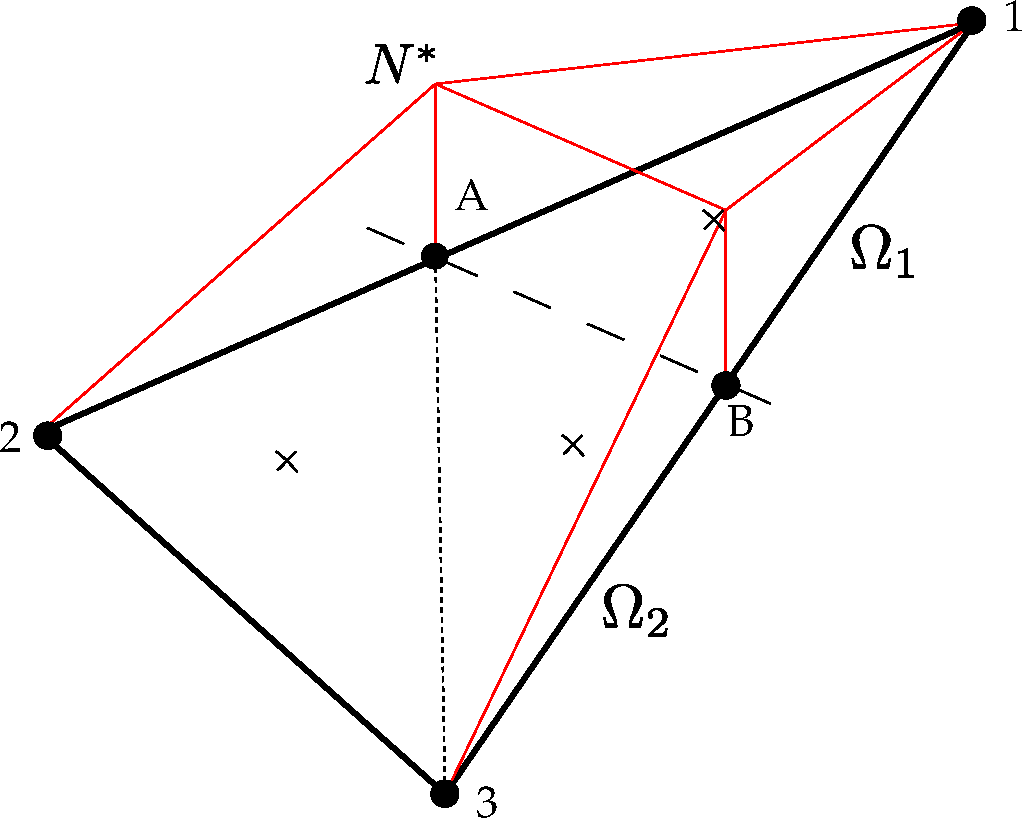
\includegraphics[width=.9\columnwidth]{images/enrichment1.pdf}
   \caption{2D interface element. The interface is calculated cutting the element with the segment $A-B$. The enrichment proposed by Coppola and the partition of the triangle into three sub-triangles with its own Gauss points to allowing to calculate an enhanced integration is shown.}
   \label{fg:enrichment1}                %% Etiqueta para la figura entera
\end{figure}

The second set of enrichment functions used in this work is described in Figure \ref{fg:enrichment2}. As in the previous case, the two new degrees of freedom can also be statically condensed. However, using this space it is possible to ensure continuity between elements, but paying the cost of having to rebuild the system matrix at each time step, which could be an expensive task due to memory allocation.
This enrichment space is constructed following
\begin{equation}
   \left\{\;
   \begin{matrix}
     \phi_A^*(\xx_A)=\phi_B^*(\xx_B)=1 \\
     \phi_A^*(\xx_1)=\phi_A^*(\xx_2)=\phi_A^*(\xx_3)=\phi_A^*(\xx_B)=0 \\
     \phi_B^*(\xx_1)=\phi_B^*(\xx_2)=\phi_B^*(\xx_3)=\phi_B^*(\xx_A)=0
   \end{matrix}\;
   \right.
   \label{eq:enrich-2a}
\end{equation}

\begin{figure}[H]
  \centering
   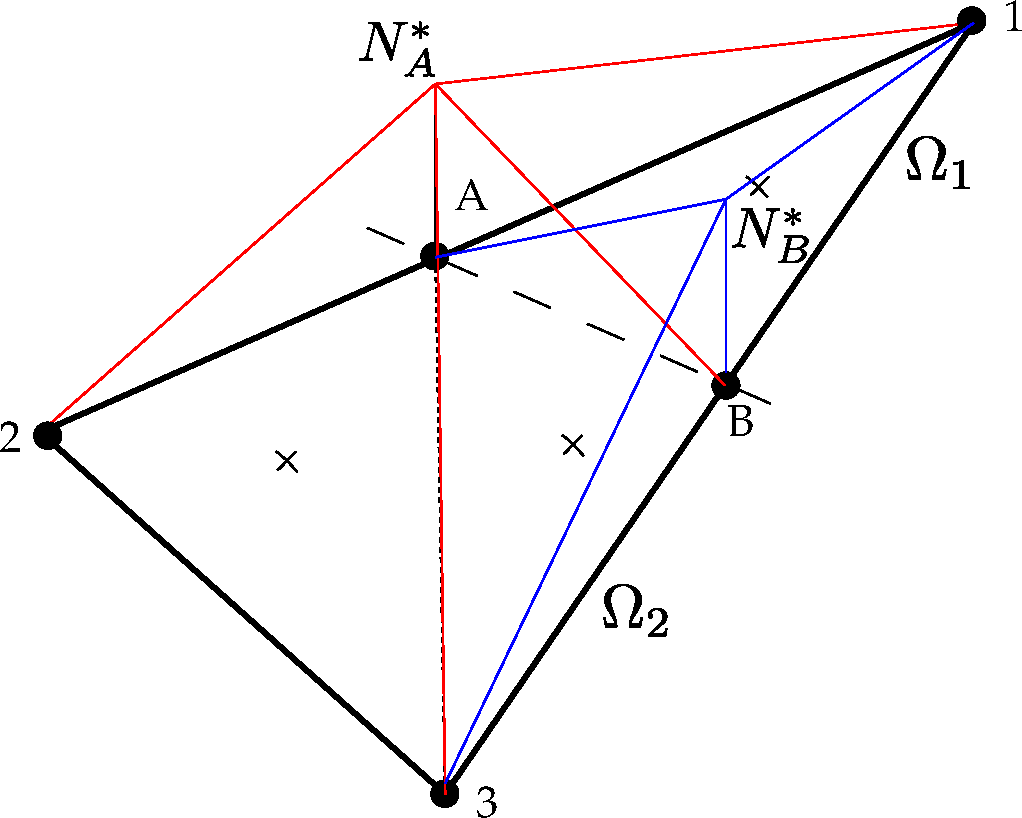
\includegraphics[width=.9\columnwidth]{images/enrichment2.pdf}
   \caption{2D interface element. The interface is calculated cutting the element with the segment $A-B$. An enrichment space with two functions per interface element, which can be used to ensure continuity between elements, is presented. The integration partition is the same as presented above (Figure \ref{fg:enrichment1}).}
   \label{fg:enrichment2}
\end{figure}

% \begin{figure}[H]
%   \centering
%     \subfloat[]{
% 	  \label{fg:enrichment1}         %% Etiqueta para la primera subfigura
% 	  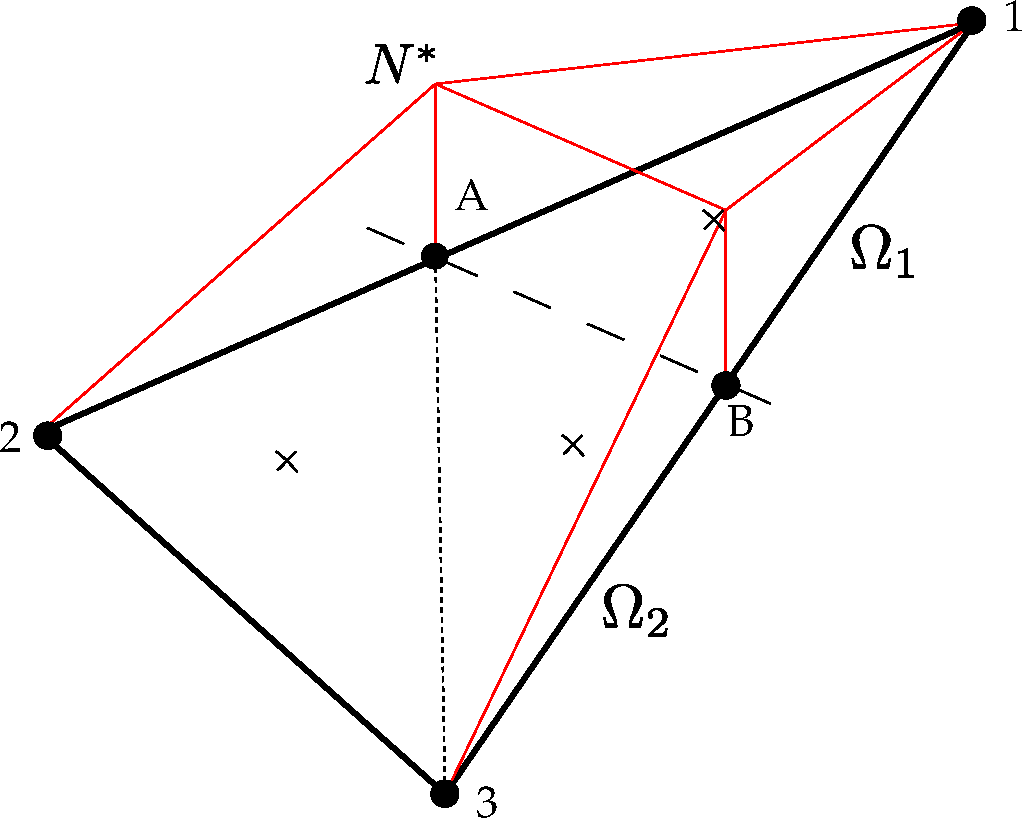
\includegraphics[width=.9\columnwidth]{images/enrichment1.pdf}
%     } \\
%     %%----segunda subfigura----
%     \subfloat[]{
% 	  \label{fg:enrichment2}         %% Etiqueta para la segunda subfigura
% 	  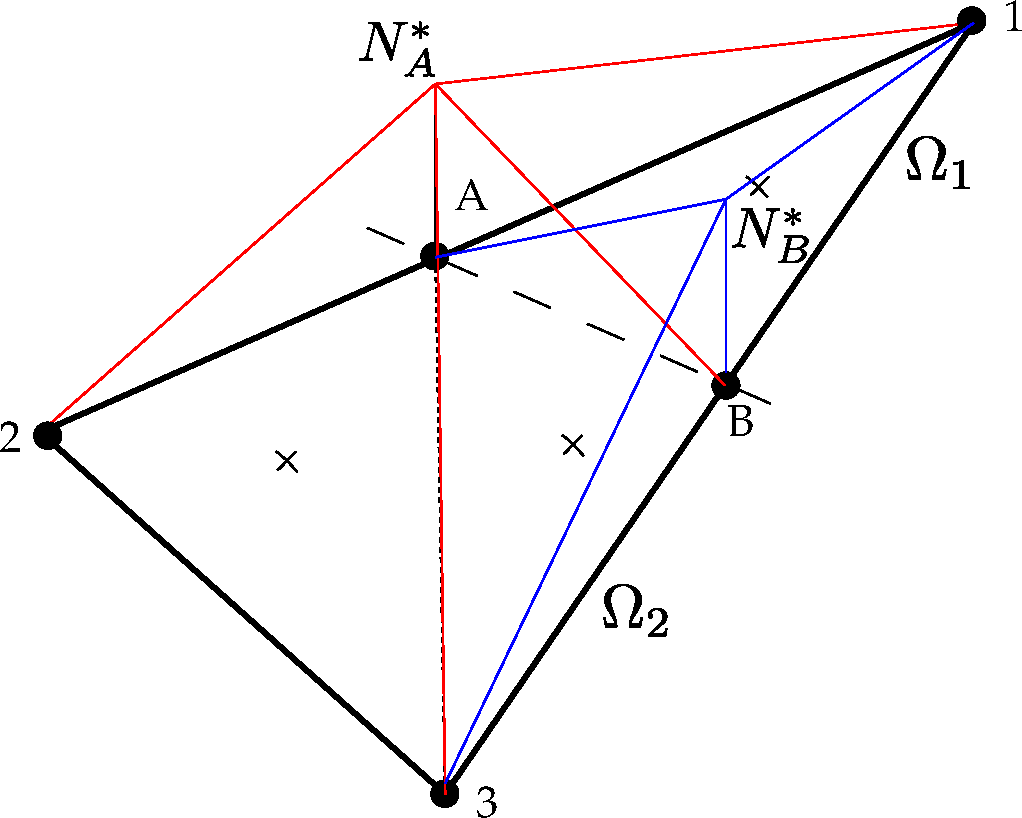
\includegraphics[width=.9\columnwidth]{images/enrichment2.pdf}
%     }
%    \caption{2D interface element. The interface is calculated cutting the element with the segment $A-B$. Figure \ref{fg:enrichment1} shows the enrichment proposed by Coppola and the partition of the triangle into three sub-triangles with its own Gauss points to allowing to calculate an enhanced integration. Figure \ref{fg:enrichment2} presents an enrichment space with two functions per interface element, which can be used to ensure continuity between elements. The integration partition is the same as presented above.}
%    \label{fg:enrichment}                %% Etiqueta para la figura entera
% \end{figure}

Therefore, using any of the enriched spaces, the pressure is now interpolated in the cut element following:
 \begin{equation}
      p_h(\xx) = \sum_{i=1}^{N_n} \phi_i(\xx) \ p_i + \sum_{i=1}^{N_e} \phi_i^*(\xx) \ p_i^*
   \end{equation}
where $\phi_i$ are traditional linear shape functions (a total of $N_n$), and $\phi_i^*$ are the enrichment shape functions (a total of $N_e$).

In order to capture the discontinuities and taking advantage of the enrichment functions used, the integration rules need to be modified in elements cut by the free surface. The method used is to divide each tetrahedra (triangular in 2D) element into up to six tetrahedral
(three triangular in 2D) sub elements. For each sub element the same integration rule as for the non-cut elements is used. Figure \ref{fg:enrichment1} shows that partition and the small circles represent the Gauss points for the integration. When using enrichment functions for the pressure, the material properties $\rho$,$\mu$ are taken as $\rho_1$,$\mu_1$ or $\rho_2$,$\mu_2$, depending on which part of the domain ($\Omega_1$ or $\Omega_2$) the integration point is found.

   \subsection{Pressure Calculation}

Particles can move across several elements and cross the interface during a time-step, consequently the pressure gradient of the previous time-step would introduce a poor and even unstable approximation of the new pressure forces. In order to avoid these large errors in the evaluation of the pressure gradients in the initial value of the iterative process, the value of the pressure is set to zero at the beginning of each time-step. Therefore, the acceleration over the particle calculated in X-IVAS stage is only is due to gravity force (pressure gradient is considered null and viscous forces are treated implicitly)\cite{Idelsohn13c}.

Starting from Equation (\ref{Step5a}), and following the classical variational formulation for the glo0bal domain $\Omega$ with boundary $\Gamma$, this is integrating, weighting with test functions and weakening both pressure laplacian and velocity divergence terms, it is possible to obtain the system:

\begin{equation}
   \left[\Delta t \int_{\Omega} \frac{1}{\rho} \nabla \phi^T \nabla \phi \ d\Omega\right]\ \delta p^{n+1} = \left[\int_{\Omega} \nabla \phi^T \psi \ d\Omega\right]\ \hat \vv_j^{n+1}
\label{poisson}
\end{equation}
where the term resulting from weakening
\begin{equation}
\displaystyle \int_{\Gamma} \phi \left[ \hat \vv_j^{n+1} + \Delta t \frac{1}{\rho} \nabla  \delta p^{n+1} \right] \cdot \mathbf{n} \ d\Gamma = \int_{\Gamma} \phi \ \vv_j^{n+1} \cdot \mathbf{n} \ d\Gamma
\end{equation}
 is zeroed to ensure impenetrability on walls.

Then, in the case of slipt elements where enrichment shape functions are used as trial functions, the resulting local system is:

  \begin{equation}
  \label{eqsys-poisson}
   \begin{pmatrix}
      L_{\phi,\phi} & L_{\phi,*}\\
      {L_{\phi,*}}^T & L_{*,*}
   \end{pmatrix}\;
    \begin{pmatrix}
      \delta p^{n+1}\\
      \delta {p^*}^{n+1}
   \end{pmatrix}\; = \;
   \begin{pmatrix}
      D_{\phi}\\
      D_*
   \end{pmatrix}\;
   (\hat{\vv}^{n+1})
\end{equation}

where
\begin{itemize}
 \item ${(L_{\phi,\phi})}_{N_n\times N_n} = \Delta t \displaystyle \int_{\Omega^e} \dfrac{1}{\rho} \nabla \phi_i^T \nabla \phi_j \ d\Omega$
 \item ${(L_{\phi,*})}_{N_n\times N_e} = \Delta t \displaystyle \int_{\Omega^e} \dfrac{1}{\rho} \nabla \phi_i^T \nabla \phi_j^* \ d\Omega$
 \item ${(L_{*,*})}_{N_e\times N_e} = \Delta t \displaystyle \int_{\Omega^e} \dfrac{1}{\rho} \nabla {\phi_i^*}^T \nabla \phi_j^* \ d\Omega$
 \item ${(D_{\phi})}_{N_n\times N_n} = \displaystyle \int_{\Omega^e} \nabla \phi_i^T \psi_j \ d\Omega$
 \item ${(D_*)}_{N_n\times N_e} = \displaystyle \int_{\Omega^e}  \nabla {\phi_i^*}^T \psi_j \ d\Omega$
\end{itemize}

At this point is possible to choose between two options. First, if the enriched space expressed by the equation (\ref{eq:enrich-2a}) is used, the new degrees of freedom can be included in the global system, which will guarantee continuity between elements. Second option is following the classical procedure of static condensation of the system through Gaussian elimination\cite{Felippa04}, where next reduced system is obtained:
  \begin{equation}
   \left[L_{\phi,\phi} - L_{\phi,*}{(L_{*,*})}^{-1}{L_{\phi,*}}^T\right](\delta p^{n+1}) = \left[D_{\phi}- L_{\phi,*}{(L_{*,*})}^{-1}D_{*}\right](\hat{\vv}^{n+1})
   \label{condensing}
  \end{equation}
with $\delta p^{n+1} = p^{n+1}-p^{n}$, where the continuity between elements is not ensured.

% --- INICIO PARRAFO IMPORTANTE A CORREGIR

In the case of enriched ones, see equation (\ref{eq:enrich-1a}), when condensation is used, the assumption of neglecting the inter-elemental boundary terms from the integration by parts of the Poisson equation is not true. From our experience, and like is reported by Coppola\cite{Coppola05}, when the Froude Number is high (this is, low density ratio), the neglected term from the weakening of the divergence of the velocity introduces severe problems of numerical diffusion.

A way to solve this problem is not integrating by parts the divergence term, but it requires imposing a pressure gradient on boundaries, whose value can not be easily predict when there is a gravitational field, low density ratio, and the fluid is not at rest.

Finally, if condensation is used, we choose weakening the velocity divergence in the Poisson step only when low density ratio is considered. Continuous enrichment does not suffer of the above mentioned problems and the same formulation can be used for every
Froude number. However, a loss of computational performance must be paid because the necessity of memory management to assemble the variable-size pressure equation system.

% --- FIN PARRAFO IMPORTANTE A CORREGIR

%   If we are interested in solving the system in absolute pressure terms, the final system is
%
%   \begin{equation}
%   [L_{\phi,\phi} - L_{\phi,*}{L_{*,*}}^{-1}{L_{\phi,*}}^T](p^{n+1}) = [D_{\phi}- L_{\phi,*}{L_{*,*}}^{-1}D_*](\hat{\vv}^{n+1}) + [L_{\phi,\phi} - L_{\phi,*}{L_{*,*}}^{-1}{L_{\phi,*}^T] (p^n)
%    \label{condensing-abs}
%   \end{equation}

After obtaining the new pressure, it is necessary to correct the velocity prediction using the pressure gradient. However, the new degree of freedom for the pressure must be taken into account in this step to calculate the enriched pressure gradient. In the case of condensed calculation, the value of $p*^{n+1}$ must be recovered from the nodal pressures calculated in the poisson step with:
\begin{equation}
  {p^*}^{n+1} = {(L_{*,*})}^{-1}[D_* \hat{\vv}^{n+1} - {L_{\phi,*}}^Tp^{n+1} + {L_{\phi,*}}^Tp^{n} + L_{*,*}{p^*}^n]
  \label{recovering}
\end{equation}

Finally, the equation system presented in Equation (\ref{correction}) must be solved.
 \begin{equation}
  \int_{\Omega} \psi \rho \vv^{n+1} d\Omega = \int_{\Omega} \psi \rho \hat{\vv}^{n+1} d\Omega - \Delta t \ \left[\int_{\Omega} \psi \nabla \delta p^{n+1} d\Omega + \int_{\Omega} \psi \nabla \delta {p^*}^{n+1} d\Omega \right]
  \label{correction}
 \end{equation}

It was previously mentioned that the pressure value is zeroed at the beginning of the time step, one of the main reason can be found in the recovering step. It must be noticed that, not only the standard nodal pressures, but also the enrichments pressures of the previous iteration are required in this stage. As the enrichment pressures depend on the interface location inside the element, using the latest $p^*$ of the previous time-step may introduce several problems due to the movement of the interface. This lead to poor results that in most cases become unstable.

Although this pressure reinitialization leads to a first order temporal approximation, successive iterations on a pressure-correction loop improve the incompressibility of the solution. Idelsohn\cite{Idelsohn13c} ensures that the stabilization effect of the first order fractional step is lost when higher order schemes are used. The same conclusion was obtained here, instead of using a stabilization technique, a limited number of iterations (two or three) were used in order to obtain a converged pressure field without any presence of pressure oscillations. More iterations would tend to make the scheme unstable. 